Raspberry pi is as such most inspiring computer available today because most devices that we use today like phones , tablets are designed in such a way that that we cannot manipulate them , From manipulation i mean we cannot design it in such a way to get a specific desired output , But raspberry is exactly opposite.
It was invented in the UK as a device for promoting the teaching of computer science and coding, and its development is overseen by The Raspberry Pi Foundation charity. The first-generation Raspberry Pi appeared in 2012 and the latest Raspberry Pi 3.0 arrived in February this year. Eight million devices have been sold worldwide, the Pi Foundation says. (Source Google).
\begin{figure}[ht]
\centering
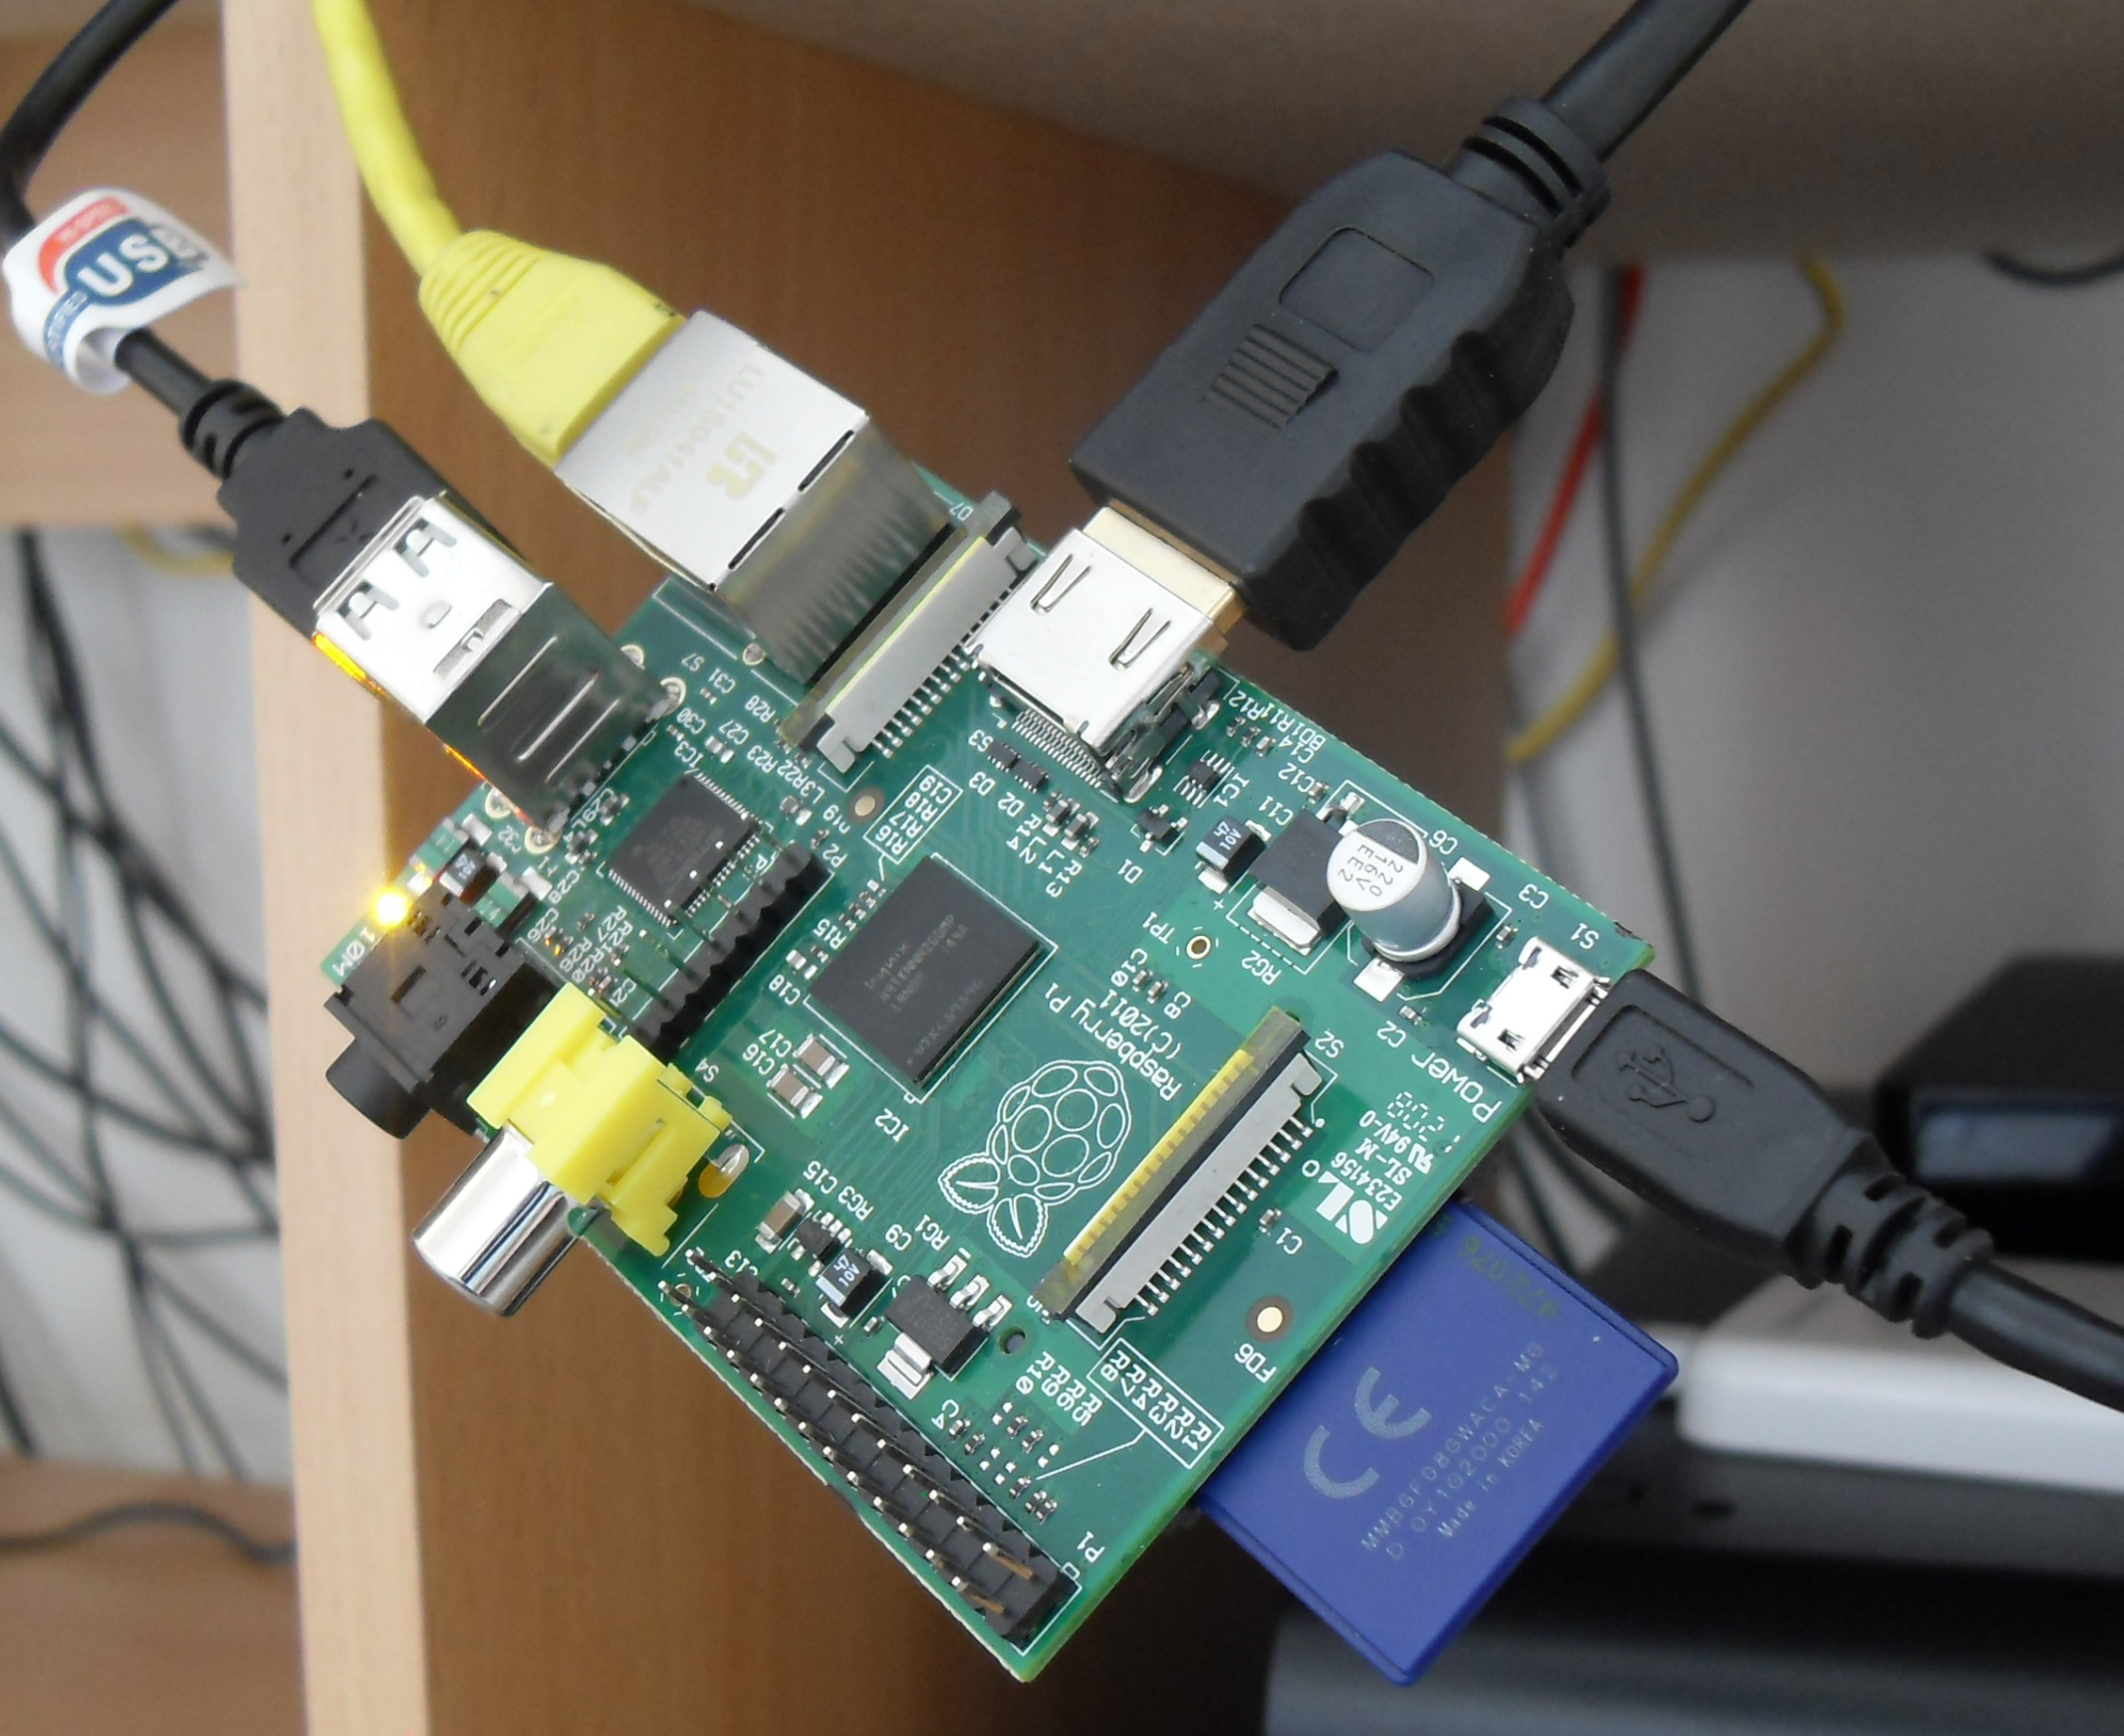
\includegraphics[scale=0.3]{images/rasp1.jpg}
\caption{Raspberry pi logo}
\end{figure}
It is credit-card sized computer which can be plugged into your TV and a keyboard , which can be used for many of the things that an  average computer does like watching movies , word processing, playing light games etc.

\section{Comparing Raspberry pi with PC}

\begin{figure}[ht]
\centering
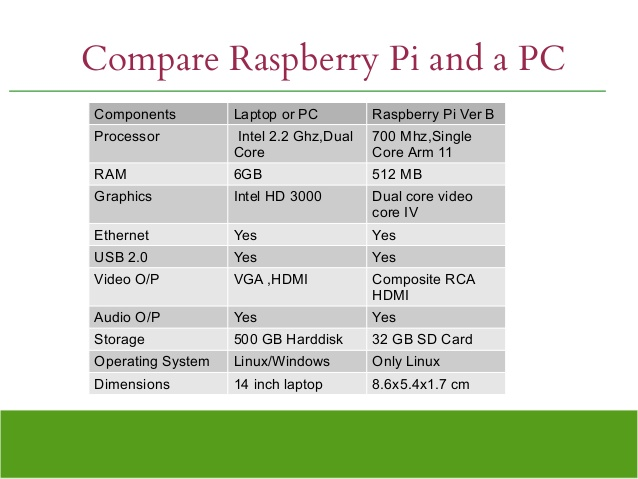
\includegraphics[scale=0.3]{images/rasp-2.png}
\caption{Raspberry pi logo}
\end{figure}
So if we compare both , In Raspberry pi we can only download open-source operating system and the Ram , Graphics and processor of Raspberry pi is comparatively low as compare to that of personal computer which works completely fine for doing basic operations other than playing high end games like GTA V.
\section{Basics of Raspberry pi}
\begin{figure}[ht]
\centering
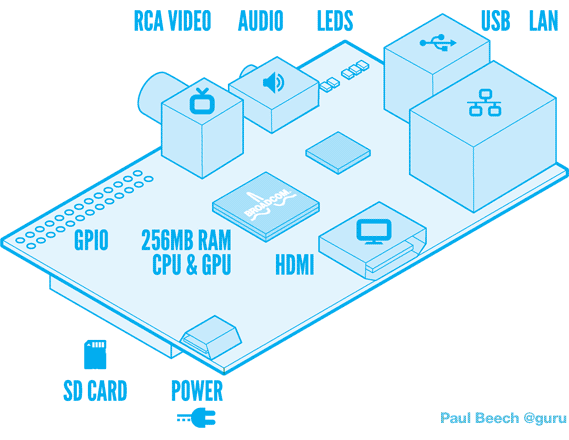
\includegraphics[scale=0.3]{images/rasp3.png}
\caption{Raspberry pi}
\end{figure}
We have HDMI port to connect raspberry pi it to monitor . We have a dedicated SD card slot for installing open-source operating system. Here we have  blue colored SD card in the picture, (in the latest version) integrated wifi and Bluetooth.
We also have a camera for recording and a headphone jack using which we can listen to songs and it  can also be useful for any automation project. We also have a 26 pin GPIO (General Purpose I/O) which is used for carrying out  specific job from  Raspberry Pie.

\section{Comparing Raspberry pie Models}
\begin{figure}[ht]
\centering
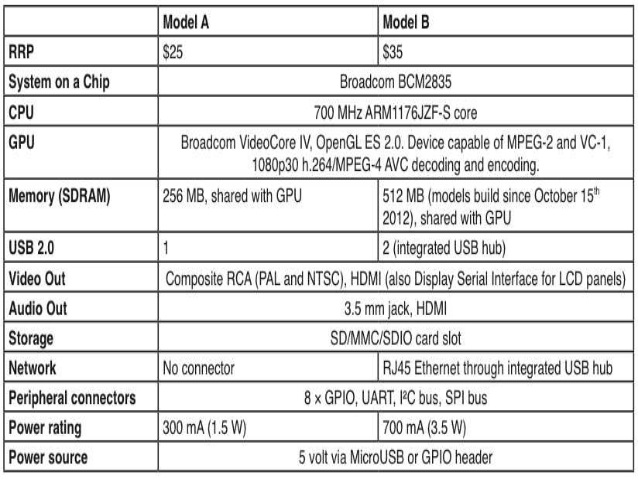
\includegraphics[scale=0.3]{images/rasp7.png}
\caption{Comparing Raspberry pie Models}
\end{figure}
There are basically two models
\begin{itemize}
\item Model A
\item Model B
\end{itemize}
It cost around \$25( ₹ 1750) for Model A and \$35 (₹ 2450) for Model B .
In Model A we don’t have Ethernet connectivity unlike in Model B where we have a RJ45 connector.
Consumption for Power in Model A ( 1.5 W) is less then that of Model B (3.5W).
\section{Operating system in Raspberry Pi}
NOOBS is a way to make setting up a Raspberry Pi for the first time much, much easier. You won’t need network access, and you won’t need to download any special imaging software. Just head to the https://www.raspberrypi.org/downloads/   page, grab a copy of the NOOBS zip file, and unpack it onto a freshly formatted 4GB (or larger) SD card. When you boot up for the first time, you’ll see a menu prompting you to install various OS’s .
\section{Why Raspberry Pi ?}
If you are a amateur computer and electronics enthusiasts who want to build their own devices this is the best thing you can get at such low cost , its definitely a value for money thing for doing automation.
You can pretty much do anything which a low powered computer can do .You can watch a movie, write a document, play basic games, and so on—it’s really up to you.
